\chapter{习题参考解答}

\section*{第1章习题 ~~\small 第\pageref{sec:ex1.1}页}

\circled{A1}-1~~证明: 
\begin{center}
	a) $(A \subset B) \Rightarrow (f(A) \subset f(B)) \nRightarrow (A \subset B)$,\qquad b) $(A \neq \varnothing) \Rightarrow (f(A) \neq \varnothing)$,
	
	c) $f(A \cap B) \subset f(A) \cap f(B)$,\qquad d) $f(A \cup B) = f(A) \cup f(B)$.
\end{center}

\circled{A1}-2~~证明: 
\begin{center}
	a) $(A' \subset B') \Rightarrow (f^{-1}(A') \subset f^{-1}(B'))$,\qquad b) $f^{-1}(A' \cap B') = f^{-1}(A') \cap f^{-1}(B')$,
	
	c) $f^{-1}(A' \cup B') = f^{-1}(A') \cup f^{-1}(B')$.
\end{center}
	
\circled{A1}-3~~证明: 
\begin{center}
	a) $f^{-1}(A'-B') = f^{-1}(A') - f^{-1}(B')$,\qquad b) $f^{-1}(Y-A') = X-f^{-1}(A')$.
\end{center} 

\circled{A1}-4~~证明: 
\begin{center}
	a) $f^{-1}(f(A)) \supset A$,\qquad b) $f(f^{-1}(B')) \subset B'$.
\end{center} 
\vspace{1em}

\circled{A2}~~证明下列命题是等价的: 

\begin{center}
	a) $f$是单射; \qquad b) $f^{-1}(f(A))=A$; \qquad c) $f(A \cap B) = f(A) \cap f(B)$;
	
	d) $f(A) \cap f(B) = \varnothing \Leftrightarrow A \cap B = \varnothing$; \qquad e) $f(A-B) = f(A) - f(B)$, 其中$B \subseteq A$. 
\end{center}
\vspace{1em}

\circled{B1}~~分别利用Schröder–Bernstein和直接构造双射证明: $[0,1]$和$(0,1)$是等势的. 
\vspace{1em}


\circled{B2}~~使用集合论公理证明von Neumann构造的自然数集$\mathbb{N}_0$中的元素满足如下性质: 
	\begin{center}
		i) $x=y \Rightarrow x^+ = y^+$; \qquad ii) $\forall x \in \mathbb{N}_0,~x^+ \neq \varnothing$;
	
		iii) $(A \subseteq \mathbb{N}_0) \wedge (\varnothing \in A) \wedge (\forall x \in A,~x^+ \in A) \Rightarrow A=\mathbb{N}_0$; \qquad iv) $x^+=y^+ \Rightarrow x=y$.
	\end{center}






\newpage
\section*{第3章习题1 ~~\small 第\pageref{sec:ex3.1}页}

\circled{A1}~~设$\lim_{n\to \infty} a_n=a$, 则$\lim_{n\to \infty} \sigma _n=a$. 

\begin{exsolution}
	通过将所有$a_n$减去$a$, 不妨令$a=0$. 任取$\varepsilon >0$, 则存在$N$使得对$n>N$均有$|a_n|<\varepsilon /2$和$\frac{1}{n} \sum_{k=1}^{N} |a_k| <\varepsilon /2$. 于是, $$|\sigma _n| \leq \frac{1}{n} \sum_{k=1}^{N} |a_k| + \frac{1}{n} \sum_{k=N+1}^{n} |a_k| < \frac{\varepsilon}{2} + \frac{\varepsilon}{2} \cdot \frac{n-N}{n} < \varepsilon .$$
\end{exsolution}

\circled{A2}~~(Silverman-Toeplitz) 若$\lim_{n\to \infty} a_n=a$, 则$\lim_{n\to \infty} b_n=a$. 

\begin{exsolution}
	通过将所有$a_n$减去$a$, 不妨令$a=0$. 注意到对任意$k$都有$t_{nk} \to 0$, 所以$\sum_{k=1}^{N} t_{nk}|a_k| \to 0$. 任取$\varepsilon >0$, 则存在$N$使得对$n>N$均有$|a_n|<\varepsilon /2$和$\sum_{k=1}^{N} t_{nk}|a_k| < \varepsilon /2$.于是, 
	$$|b_n| \leq \sum_{k=1}^{N} t_{nk} |a_k| + \sum_{k=N+1}^{n}t_{nk}|a_k| < \frac{\varepsilon}{2} + \frac{\varepsilon}{2}\sum_{k=N+1}^{n}t_{nk} < \varepsilon .$$
\end{exsolution}

\circled{A3}~~(Stolz-Cesáro) 设数列$\{ a_n \}$和$\{ b_n \}$, 其中$\{ b_n \}$严格递增, 且$\lim_{n\to \infty} b_n = \infty$. 那么$$\lim_{n\to \infty} \frac{a_n}{b_n} = \lim_{n\to \infty} \frac{a_n-a_{n-1}}{b_n-b_{n-1}}. $$
(前提是右侧极限存在且为实数)

\begin{exsolution}
	\underline{\textbf{方法一}}~~构造Toeplitz矩阵$T=(t_{nk})$, 其中$t_{nk}=\frac{b_k-b_{k-1}}{b_n}$, 容易验证这样的定义符合要求. 记$x_n = \frac{a_n-a_{n-1}}{b_n-b_{n-1}}$, 则$$\lim_{n\to \infty} \sum_{k=1}^{n} t_{nk}x_k = \lim_{n\to \infty} \sum_{k=1}^{n} \frac{a_k-a_{k-1}}{n_n} =\lim_{n\to \infty} \frac{a_n}{b_n} = \lim_{n\to \infty} x_n. $$
	
	\underline{\textbf{方法二}}~~只需证明$$\liminf_{n\to \infty} \frac{a_n-a_{n-1}}{b_n-b_{n-1}} \leq \liminf_{n\to \infty} \frac{a_n}{b_n} \leq \limsup_{n\to \infty} \frac{a_n}{b_n} \leq \limsup_{n\to \infty} \frac{a_n-a_{n-1}}{b_n-b_{n-1}}.$$
	
	以右侧为例. 记$s = \limsup_{n\to \infty} \frac{a_n-a_{n-1}}{b_n-b_{n-1}}$. 任取$s_1>s$, 存在$N$使得任意$n>N$有$\frac{a_n-a_{n-1}}{b_n-b_{n-1}} <s_1$, 从而$$\frac{a_n-a_{N-1}}{b_n-b_{N-1}} \leq \max \big\{ \frac{a_N-a_{N-1}}{b_N-b_{N-1}},\cdots ,\frac{a_n-a_{n-1}}{b_n-b_{n-1}} \big\} < s_1. $$
	上式化简可得$$\frac{a_n}{b_n} < s_1\ssb{1-\frac{b_{N-1}}{b_n}} + \frac{a_{N-1}}{b_n}. $$
	两侧同时令$n\to \infty$有$\limsup_{n\to \infty} \frac{a_n}{b_n} \leq s_1$. 再令$s_1\to s$则可证原式成立. 
\end{exsolution}

\circled{B1}~~证明, 数列$\{ x_n \}$上下极限的三种定义方式是等价的: (以下极限为例)

a) $\liminf_{k\to \infty} x_k:=\lim_{n\to \infty} \inf_{k \geq n} x_k$;\qquad b) $\liminf_{k\to \infty} x_k:= \min  \{\{ x_n \}\text{的聚点} \}$; 

c) $\liminf_{k\to \infty} x_k:= \sup \{ a\in \R \cup \{ -\infty \}: \forall \varepsilon >0, \exists N \in \mathbb{N}^{*} (\forall n>N, x_n>a-\varepsilon ) \}$

\begin{exsolution}
	a) $\Rightarrow$ b): 已经在讲义中证明过了. 
	
	b) $\Rightarrow$ c): 记$i=\min  \{\{ x_n \}\text{的聚点} \}$, $E = \{ a\in \R \cup \{ -\infty \}: \forall \varepsilon >0, \exists N \in \mathbb{N}^{*} (\forall n>N, x_n>a-\varepsilon ) \}$. 
	
	若数列有下界. 先证明$i \leq \sup E$: 若不然, 即存在$\varepsilon >0$使得存在无穷多个$x_n$使得$x_n+\varepsilon >i$, 进而由Bolzano-Weierstrass定理, $(-\infty ,i-\varepsilon)$中存在聚点, 这与$i$的定义矛盾. 
	
	再证明$i \geq \sup E$: 若不然, 即存在$a \in E$使得$a>i$, 进而存在$\varepsilon >0$使得$a-\varepsilon >i$. 针对该$\varepsilon$, 存在$N$使得任意$n>N$都有$x_n>a-\varepsilon$, 说明$(-\infty ,a-\varepsilon)$中只有有限项, 故不存在聚点, 矛盾. 
	
	若数列无下界, 显然$i=-\infty$, 同时$E=\{ -\infty \}$. 
	
	c) $\Rightarrow$ a): 若数列有下界. 先证明$i \leq \lim_{n\to \infty} i_n$: 由定义, 任取$\varepsilon >0$, 存在$N$使得当$n>N$时$x_n > i-\varepsilon$, 进而$i_n > i-\varepsilon$, 取极限可知$\lim_{n\to \infty} i_n \geq i-\varepsilon$. 从而$i \leq \lim_{n\to \infty} i_n$. 
	
	再证明$i \geq \lim_{n\to \infty} i_n$. 若否, 存在$N$使得当$n>N$时$i<i_n$, 则此时$E \cap \{ x_n \}_{n>N} = \varnothing$. 即存在$\varepsilon >0$使得对任意$k>N$, $x_k > x_n-\varepsilon$, 矛盾. 
\end{exsolution}

\circled{B2}~~设数列$\{ a_n \}, \{ b_n \}$, 则其下极限是超可加的, 上极限是次可加的, 即
\begin{align*}
	\underline{\liminf_{n\to \infty} a_n + \liminf_{n\to \infty} b_n \leq \liminf_{n\to \infty} (a_n+b_n) }&\leq \liminf_{n\to \infty} a_n + \limsup_{n\to \infty} b_n \\
	&\leq \underline{\limsup_{n\to \infty} (a_n+b_n) \leq \limsup_{n\to \infty} a_n + \limsup_{n\to \infty} b_n}.
\end{align*}

特别地, $$\liminf_{n\to \infty} (a_n+b_n)  = \lim_{n\to \infty} a_n + \liminf_{n\to \infty} b_n , \qquad \limsup_{n\to \infty} (a_n+b_n)  = \lim_{n\to \infty} a_n + \limsup_{n\to \infty} b_n. $$

\begin{exsolution}
	以左侧为例. 对于$n$, 任取$l >n$, 则$\inf_{k \geq n}a_k \leq a_l, \inf_{k \geq n}b_k \leq a_l$, 从而$\inf_{k \geq n}a_k + \inf_{k \geq n}b_k \leq \inf_{k \geq n}(a_k+b_k)$. 两侧对$n$取极限即得左边不等式. 
	
	进一步地, $\inf_{k \geq n}a_k + \sup_{k \geq n}b_k \geq \inf_{k \geq n}(a_k+b_k) + \inf_{k \geq n}(-b_k) + \sup_{k \geq n}b_k = \inf_{k \geq n}(a_k+b_k)$. 同上可得中间不等式. 
\end{exsolution}

\circled{B3}-1~~设非负数列$\{ a_n \}, \{ b_n \}$, 类似于B2有如下结论: 
\begin{align*}
	\underline{\ssb{\liminf_{n\to \infty} a_n}\ssb{ \liminf_{n\to \infty} b_n} \leq \liminf_{n\to \infty} (a_nb_n) } &\leq \ssb{\liminf_{n\to \infty} a_n}\ssb{ \limsup_{n\to \infty} b_n} \\
	&\leq \underline{\limsup_{n\to \infty} (a_nb_n) \leq \ssb{\limsup_{n\to \infty} a_n}\ssb{ \limsup_{n\to \infty} b_n}}.
\end{align*}

\begin{exsolution}
	以左侧为例. 同B2可证$\ssb{\inf_{k\geq n}a_n} \ssb{\inf_{k\geq n}b_n} \leq \inf_{k\geq n}(a_nb_n)$. 任取$\varepsilon >0$, 存在$\ell \geq n$使得$a_{\ell} < \varepsilon + \inf_{k\geq n} a_k$, 又$b_{\ell} \leq \sup_{k\geq n}b_k$, 故$$\ssb{\varepsilon + \inf_{k\geq n} a_k} \ssb{\sup_{k\geq n}b_k} >a_{\ell}b_{\ell} \geq \liminf_{n\to \infty} (a_nb_n). $$
	令$\varepsilon \to 0$即得所需不等式. 最后令$n\to \infty$可证原命题成立. 
\end{exsolution}

\circled{B3}-2~~特别地, 对非负数列$\{ a_n \}$和任意数列$\{ b_n \}$都有$$\liminf_{n\to \infty} (a_nb_n) = \ssb{\lim_{n\to \infty} a_n} \ssb{\liminf_{n\to \infty} b_n}, \qquad \limsup_{n\to \infty} (a_nb_n) = \ssb{\lim_{n\to \infty} a_n} \ssb{\limsup_{n\to \infty} b_n}.$$

\begin{exsolution}
	以上极限为例. 记$\limsup_{n\to \infty} b_n=s$, $\lim_{n\to \infty} a_n =a$. 
	
	若$s>0$, 令$b_n^+=\frac{|b_n|+b_n}{2} \geq 0$, 且$\limsup_{n\to \infty} b_n^+ = s$. 易见$as = \limsup_{n\to \infty}(a_nb_n^+) = \limsup_{n\to \infty}(a_nb_n)$. 
	
	若$s \leq 0$, 存在$\varepsilon >0$使得$s + \varepsilon >0$, 令$b_n' = b_n+\varepsilon$. 应用B3-2和B2可以得到$$\limsup_{n\to \infty}(a_nb_n+\varepsilon a_n) = a\limsup_{n\to \infty} (b_n+\varepsilon) \quad \Rightarrow \quad  \limsup_{n\to \infty} (a_nb_n) + \varepsilon a = \limsup_{n\to \infty} b_n + \varepsilon a. $$
\end{exsolution}

\circled{B4}~~设正数列$\{ a_n \}$, 则$$\liminf_{n\to \infty} \frac{a_{n+1}}{a_n} \leq \liminf_{n\to \infty} \sqrt[n]{a_n} \leq \limsup_{n\to \infty} \sqrt[n]{a_n} \leq \limsup_{n\to \infty} \frac{a_{n+1}}{a_n}. $$

\begin{exsolution}
	以右侧为例. 记$s=\limsup_{n\to \infty} \frac{a_{n+1}}{a_n}$. 对任意$\varepsilon >0$, 存在$N$使得对任意$n>N$都有$\frac{a_{n+1}}{a_n} \leq s+\varepsilon$, 这就是说$a_n \leq (s+\varepsilon)^{n-N}a_N$, 进而$$\sqrt[n]{a_n} \leq (s+\varepsilon) \sqrt[n]{\frac{a_N}{(s+\varepsilon)^N}} \to s+\varepsilon ,\quad n \to \infty .$$
	再由$\varepsilon >0$取值的任意性可得$\limsup_{n\to \infty} \sqrt[n]{a_n} \leq s$. 
\end{exsolution}







\newpage
\section*{第3章习题2 ~~\small 第\pageref{sec:ex3.2}页}

\circled{A1}-1~~证明$\rm exp$是定义良好的. 

\begin{exsolution}
	显见, 对足够大的$k$均有$|\frac{z^k}{k!} | \leq \frac{1}{2^k}$. 
\end{exsolution}

\circled{A1}-2~~用级数定义的指数函数$\rm \exp$满足: 对任意的$z_1,z_2 \in \C$, ${\rm exp}(z_1+z_2) = {\rm exp} (z_1) \cdot {\rm exp} (z_2)$. 

\begin{exsolution}
	注意到: $$e^{z_1}\cdot e^{z_2}& = (\sum_{k=0}^\infty \frac{z_1^k}{k!})(\sum_{k=0}^\infty \frac{z_2^k}{k!}) = \sum_{k=0}^\infty \sum_{i+j=k}\frac{z_1^i}{i!}\frac{z_2^j}{j!} = \sum_{k=0}^\infty\frac{1}{k!} \sum_{i+j=k}\frac{k!}{i!j!} z_1^i \cdot z_2^j = \sum_{k=0}^\infty\frac{1}{k!}(z_1+z_2)^k=e^{z_1+z_2}.$$
\end{exsolution}

\circled{A2}-1~~对任意$z \in \C$, 都有$(\cos z)^2+(\sin z)^2=1$. 特别地有$|\sin z| \leq 1$和$|\cos z| \leq 1$. 

\begin{exsolution}
	直接验证即可. 
\end{exsolution}

\circled{A2}-2~~三角函数的和差角公式: 对任意$x,y \in \C$, $$\cos(x+y) = \cos x \cos y - \sin x \sin y,\qquad \sin(x+y) = \sin x \cos y + \cos x \sin y.$$

\begin{exsolution}
	利用$e^{\ic x+ \ic y}=e^{\ic x} \cdot e^{\ic y}$, 比较两边系数即可. 
\end{exsolution}






\newpage
\section*{第3章习题3 ~~\small 第\pageref{sec:ex3.3}页}

\circled{A1}~~证明: 存在唯一的函数$f: \R \to \R $满足: $$f(1)=a , \qquad \forall x,y \in \R , f(x)+ f(y) = f(x+y),\qquad \textit{$f(x)$在$\R$上单调递增}.$$

\circled{A2}~~证明: 存在唯一的函数$f: \R \to \R $满足: $$f(1)=a ~(a>0,a \neq 1), \qquad \forall x,y \in \R , f(x)\cdot f(y) = f(x+y),\qquad \forall x_0 \in \R, \lim_{x \to x_0} f(x)=f(x_0).$$

\circled{B1}~~设正项级数$\sum_{n=1}^{\infty} a_n, \sum_{n=1}^{\infty} b_n$, 且当$n\to \infty$时$a_n \sim b_n$, 则这两个级数敛散性相同. 以此证明, $\sum_{n=1}^{\infty} \sin (1/n^p)$在$p>1$时收敛. 
\vspace{1em}

\circled{B2}-1~~若对任意$n \in \mathbb{N}^*$都有$a_n \geq a_{n+1}>0$且级数$\sum_{n=1}^{\infty} a_n$收敛, 则当$n\to \infty$时$a_n=o(1/n)$. 
\vspace{1em}

\circled{B2}-2~~若$b_n=o(1/n)$, 总存在数列$a_n$使得级数$\sum_{n=1}^{\infty} a_n$收敛且当$n\to \infty$时$b_n=o(a_n)$. 
\vspace{1em}

\circled{B3}-1~~若正项级数$\sum_{n=1}^{\infty} a_n$收敛, 那么级数$\sum_{n=1}^{\infty} A_n$亦收敛, 并且当$n\to \infty$时$a_n=o(A_n)$. 其中$$A_n=\sqrt{\sum_{k=n}^{\infty} a_k} - \sqrt{\sum_{k=n+1}^{\infty} a_k}.$$

\circled{B3}-2~~若正项级数$\sum_{n=1}^{\infty} a_n$收敛, 那么级数$\sum_{n=2}^{\infty} A_n$亦收敛, 并且当$n\to \infty$时$A_n=o(a_n)$. 其中$$A_n=\sqrt{\sum_{k=1}^{n} a_k} - \sqrt{\sum_{k=1}^{n-1} a_k}.$$

\circled{B4}-1~~若$\frac{b_n}{b_{n+1}}=1+\beta _n$对所有$n \in \mathbb{N}^*$成立, 且级数$\sum_{n=1}^{\infty} \beta _n$绝对收敛, 则$\lim_{n\to \infty} b_n$存在. 
\vspace{1em}

\circled{B4}-2~~若$\frac{a_n}{a_{n+1}}=1+\frac{p}{n} +\alpha _n$对所有$n \in \mathbb{N}^*$成立, 且级数$\sum_{n=1}^{\infty} \alpha _n$绝对收敛, 则当$n\to \infty$时$a_n \sim c/n^p$. 
\vspace{1em}

\circled{B4}-3~~(Gauss判别法) 若数列$\{ a_n \}$满足$\frac{a_n}{a_{n+1}}=1+\frac{p}{n} +\alpha _n$对所有$n \in \mathbb{N}^*$成立, 且级数$\sum_{n=1}^{\infty} \alpha _n$绝对收敛, 那么$\sum_{n=1}^{\infty} a_n$在$p>1$时绝对收敛, 反之发散. 
\vspace{1em}

\circled{B5}~~证明对任意正项数列$\{ a_n \}$都有{\color{blue}最优}估计
\begin{center}
	$\displaystyle \limsup_{n\to \infty} \left(\frac{1+a_{n+1}}{a_n} \right)^n \geq e.$
\end{center}

\circled{C1}~~(Cauchy判别准则) $\prod_{n \geq 1}a_n$收敛当且仅当对任意的$\varepsilon >0$, 存在$N$使得任意的$n \geq N$和任意的$p \geq 0$有$$|a_n \cdot \cdots \cdot a_{n+p}-1|<\varepsilon .$$

\circled{C2}~~设$\{ a_n \}$是正实数序列, 则无限乘积$\prod_{n \geq 1} (1+a_n)$收敛当且仅当级数$\sum_{n\geq 1}a_n$收敛. 特别地, 对于复数列$\{ b_n \}$, 若$\sum_{n\geq 1}b_n$绝对收敛, 则$\prod_{n \geq 1} (1+|b_n|)$收敛, 进而$\prod_{n \geq 1} (1+b_n)$收敛. 
\vspace{1em}

\circled{C3}~~计算: $$\prod_{n=1}^{\infty} \ssb{1+x^{2^{n-1}}},\qquad \prod_{n=1}^{\infty} \cos \frac{x}{2^n}.$$

\circled{C4}-1~~设$\mathcal{P}$是所有素数构成的集合. 对于$s>1$, $\zeta$-函数$$\zeta (s) = \sum_{n=1}^{\infty} \frac{1}{n^s}$$
是良好定义的, 并且$$\zeta (s) = \prod_{p \in \mathcal{P}} \frac{1}{1-p^{-s}}. $$

\circled{C4}-2~~利用按$2^k$为长度分组放缩的方式, 可以得到$\zeta (s)$的下界估计: $$\zeta (s) \geq \sum_{k=1}^{\infty} \frac{1}{2^{ks}} \times 2^{k-1} = \frac{1/2}{1-\frac{1}{2^{s-1}}}.$$
从而当$s \to 1$时$\zeta (s) \to \infty$. 借此证明: $\mathcal{P}$是无限集合. 









\newpage
\section*{第4章习题 ~~\small 第\pageref{sec:ex4.1}页}

\circled{A1}~~设$f,g \in C([a,b])$, 则存在$x_0 \in [a,b]$使得$d(f,g) = |f(x_0)-g(x_0)|$. 

\begin{exsolution}
	只需注意到$|f(x)-g(x)|$连续即可. 
\end{exsolution}

\circled{A2}-1~~零次最佳逼近多项式存在. 

\begin{exsolution}
	取$P_0(x)=\frac{1}{2}(\sup_{x \in [a,b]} f(x) + \inf_{x \in [a,b]} f(x))$即可. 
\end{exsolution}

\circled{A2}-2~~当$P_n$是固定的多项式时, 存在$\lambda _0$使得$d(f,\lambda _0P_n) = \inf_{\lambda \in \R} d(f,\lambda P_n)$. 

\circled{A2}-3~~若$n$次最佳逼近多项式存在, 则$n+1$次最佳逼近多项式也存在. 

\circled{A3}~~(Vallée Poussin) 如果在闭区间$[a,b]$上有$n+2$个点$x_0 <\cdots <x_{n+1}$, 使得量$\sgn \big( (f(x_i)-P(x_i))(-1)^i \big)$在$i=0,\cdots ,n+1$时为常数, 则$E_n(f) \geq \min_{0 \leq i \leq n+1} |f(x_i)-P_n(x_i)|$. 
\vspace{1em}

\circled{A4}-1~~(Chebyshev) 若$P_n(x)$是$f \in C([a,b])$的$n$次最佳逼近多项式, 则在闭区间$[a,b]$上可以求出至少$n+2$个Chebyshev交错点. {\color{blue}该命题的证明需要用到很多引理, 没有做的必要, 后文可以直接使用. }

\circled{A4}-2~~求$f(x)=x^2$在$[0,1]$上的$1$次最佳逼近多项式, 并以此构造反例说明当$f$不连续时上述命题不一定成立. 

\circled{A4}-3~~若在$[a,b]$上可以求出至少$n+2$个Chebyshev交错点, 则$P_n(x)$是$f \in C([a,b])${\color{blue}唯一}的$n$次最佳逼近多项式. 

\circled{A5}~~在$x^n$的系数为$1$的多项式中, 多项式$T_n(x)/2^{n-1}$是$f(x)=0, -1 \leq x \leq 1$的最佳逼近多项式. 

\begin{figure}[H]
	\centering
	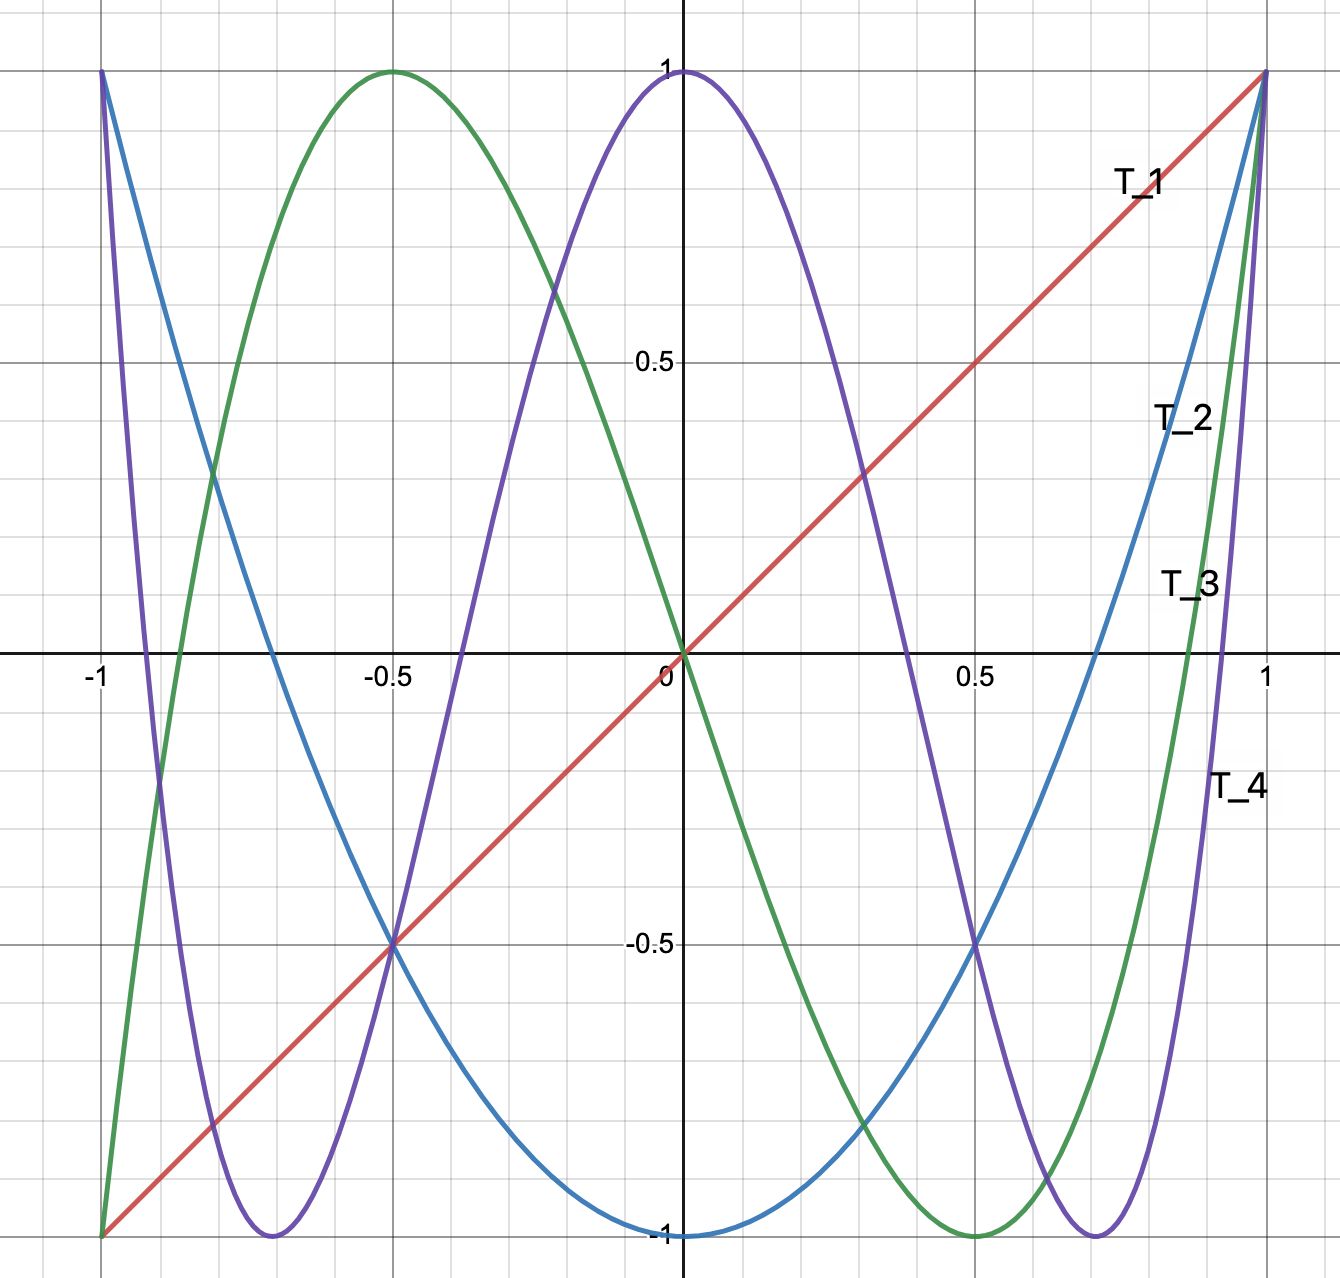
\includegraphics[width=7cm]{attachment/iShot_2024-02-01_18.43.57.png}
	\caption{$T_1 \sim T_4$在$[-1,1]$上的示意图}
\end{figure}







\newpage
\section*{第6章习题1 ~~\small 第\pageref{sec:ex6.1}页}

\circled{A1}-1~~设$f \in C^{n-1}([a,b])$, 且在$(a,b)$上存在$n$阶导数. 设$x_0+h_1,\cdots ,x_0+h_1+\cdots +h_n$均包含于$[a,b]$, 那么存在包含这些点的最小闭区间内的点$\xi$使得$$\Delta ^n f(x_0;h_1,\cdots ,h_n) = f^{(n)}(\xi) h_1\cdots h_n. $$
\begin{exsolution}
	用归纳法. 当$n=1$时该命题即为Lagrange中值定理. 假设对任意$k \leq n-1$命题均成立, 则存在$\xi$使得$$\Delta ^n f(x_0;h_1,\cdots ,h_n) = \Delta ^{n-1}g(x_0;h_1,\cdots ,h_{n-1}) = g^{(n-1)}(\xi) h_1\cdots h_{n-1}. $$
	其中$g(x)=f(x+h_n)-f(x)$. 由Lagrange中值定理, 存在$\tilde{\xi}$使得$$g^{(n-1)}(\xi) = f^{(n-1)}(\xi + h_n) - f^{(n-1)}(\xi) = f^{(n)}(\tilde{\xi}). $$
	将两式相乘, 即得原命题成立. 另外不难验证$\tlde{\xi}$的取值范围. 
\end{exsolution}

\circled{A1}-2~~特别地, 记$\Delta ^nf(x_0;h^n) := \Delta ^nf(x_0;h,\cdots ,h)$. 若$f^{(n)}(x_0)$存在, 则$$f^{(n)}(x_0) = \lim_{h \to 0} \frac{\Delta ^n f(x_0;h^n)}{h^n}. $$
\begin{exsolution}
	用归纳法. 当$n=1$时即为导数定义. 假设对任意$k \leq n-1$命题均成立, 则$$\lim_{h \to 0} \frac{\Delta ^n f(x_0;h^n)}{h^n} = \lim_{h \to 0} \frac{\Delta ^{n-1} g(x_0;h^{n-1})}{h^{n-1}} = \lim_{h\to 0} \frac{\Delta ^{n-1}f'(x_0;h^{n-1})}{h^{n-1}} = f^{(n)}(x). $$
	其中$g(x) = \frac{f(x+h)-f(x)}{h}$. 
\end{exsolution}

\circled{A1}-3~~函数$f(x)=\begin{cases}
	x^3\sin \frac{1}{x} & x\neq 0 \\ 0 & x = 0
\end{cases}$满足$\displaystyle \lim_{h\to 0} \frac{\Delta ^2 f(0;h^2)}{h^2}$存在但$f^{(2)}(0)$不存在. 
\begin{exsolution}
	计算可知$$\frac{\Delta ^2 f(0;h^2)}{h^2} = 8h\sin \frac{1}{2h} - 2h\sin \frac{1}{h} \leq 2h^3\left(4\sin \frac{1}{2h} - \sin \frac{1}{h} \right) \to 0,\quad h\to 0. $$
	但是$$f'(x) = \begin{cases}
		3x^2\sin \frac{1}{x} - x\cos \frac{1}{x} & x \neq 0 \\ 0 & x=0
	\end{cases},\qquad f''(0)=\lim_{h\to 0} \left( 3h\sin \frac{1}{h}-\cos \frac{1}{h} \right)~\textit{不存在}.$$
\end{exsolution}

\circled{B1}-1~~若将$I$依次分为区间$I_1,I_2,I_3$, 则$$m_k(I) \leq \frac{1}{|I_2|} (m_{k-1}(I_1) + m_{k-1}(I_3)). $$
\begin{exsolution}
	任取$x \in I_1$和$y \in I_3$, 由Lagrange中值定理, 存在$\xi \in (x,y)$使得$$|f^{(k)}(\xi)| = \frac{|f^{(k-1)}(x)-f^{(k-1)}(y)|}{|x-y|} \leq \frac{|f^{(k-1)}(x)|+|f^{(k-1)}(y)|}{|I_2|}. $$
	由$x,y$选取的任意性可知$$\frac{1}{|I_2|} (m_{k-1}(I_1) + m_{k-1}(I_3)) \geq |f^{(k)}(\xi _{x,y})| \geq m_k(I). $$
\end{exsolution}

\circled{B1}-2~~记$\lambda = |I|$, 则$$m_k(I) \leq \frac{2^{\frac{k(k+1)}{2}} k^k}{\lambda ^k}. $$
\begin{exsolution}
	用归纳法. 当$k=1$时, 对任意分划, 注意到$$m_1(I) \leq \frac{1}{|I_2|} (\inf_{x \in I_1} |f(x)| + \inf_{x \in I_3} |f(x)|) \leq \frac{2}{\lambda}. $$
	假设命题对任意小于$k$的自然数成立, 则$$m_k(I) \leq \frac{1}{|I_2|} (m_{k-1}(I_1)+m_{k-1}(I_3)) \leq \frac{1}{|I_2|} 2^{ \frac{(k-1)k}{2} }(k-1)^{k-1} \left( \frac{1}{|I_1|^{k-1}} + \frac{1}{|I_3|^{k-1}}  \right). $$
	于是只需要证明$$\frac{1}{|I_2|} \left( \frac{1}{|I_1|^{k-1}} + \frac{1}{|I_3|^{k-1}} \right) \leq \frac{(2k)^k}{\lambda ^k(k-1)^{k-1}}. $$
	利用$|I_1|+|I_2|+|I_3|=\lambda$即可求导证明. 
\end{exsolution}

\circled{B1}-3~~存在只与$n$有关的$\alpha _n$, 使得若$|f'(0)| \geq \alpha _n$, 则$f^{(n)}(x)$在$(-1,1)$上有至少$n-1$个不同的零点. 
\begin{exsolution}
	假设已经找到了这样的$\alpha _n$, 下用归纳法证明: 对任意$k \leq n$都存在$x_k^1<\cdots <x_k^k$使得$x_k^k-x_k^1 \leq d_k$, 且对任意$j=1,\cdots ,k$都有$\sigma (-1)^{j} f^{(k)}(x_k^j) \geq \ell _k >0$, 其中$\ell _k,d_k$待定. 
	
	归纳的第一步待定. 现在假设命题对任意小于$k$的自然数均成立. 
	
	先构造$x_k^2,\cdots ,x_k^{k-1}$: 由Lagrange中值定理, 存在$x_k^j \in (x_{k-1}^{j-1},x_{k-1}^{j})$使得
	
	$$f^{(k)}(x_k^j) = \frac{f^{(k-1)}(x_{k-1}^{j}) - f^{(k-1)}(x_{k-1}^{j-1})}{x_{k-1}^{j}-x_{k-1}^{j-1}}. $$
	显然这样构造出来的$x_k^2,\cdots ,x_k^{k-1}$(的函数值)满足正负交错排列的要求. 对$f^{k-1}(x_{k-1}^{j})$的正负分类讨论可知$$|f^{(k)}(x_k^j)| \geq \frac{2\ell _{k-1}}{x_{k-1}^{j}-x_{k-1}^{j-1}} \geq \frac{2\ell _{k-1}}{d_{k-1}}. $$
	于是需要令$\ell _k \leq \frac{2\ell _{k-1}}{d_{k-1}}$. 
	
	接着构造$x_k^1,x_k^{k}$. 以$x_k^1$为例, 待定$\delta _{k-1}$使得$I_1=(x_{k-1}^1-\delta _{k-1},x_{k-1}^1) \subseteq I$(这里需要有$d_k \geq d_{k-1}+2\delta _k$). 那么由上一问可知存在$x_{k-1}^{0} \in I_1$使得$$|f^{k-1}(x_{k-1}^{0})| \leq \frac{2^{ \frac{(k-1)k}{2} } (k-1)^{k-1}}{\delta _{k-1}^{k-1}}. $$
	由Lagrange中值定理可知存在$x_k^1 \in (x_{k-1}^{0},x_{k-1}^{1})$使得$$f^{(k)}(x_k^1) = \frac{f^{(k-1)}(x_{k-1}^1) - f^{(k-1)}(x_{k-1}^0)}{x_{k-1}^1 - x_{k-1}^0}. $$
	当$|f^{k-1}(x_{k-1}^{0})|$比较小时, $x_k^1$与$x_k^2$(的函数值)可以正负交错. 另外$$|f^{(k)}(x_k^k)| \geq \frac{|f^{(k-1)}(x_{k-1}^1)| - |f^{(k-1)}(x_{k-1}^0)|}{x_{k-1}^1 - x_{k-1}^0} \geq \frac{\ell _{k-1} - \frac{2^{ \frac{(k-1)k}{2} } (k-1)^{k-1}}{\delta _{k-1}^{k-1}}}{\delta _{k-1}}. $$
	于是需要令$\ell _k \leq RHS$. 
	
	综合上述分析, 不难猜到$\delta _k \to 0$, $d_k \to |I|$, 于是令$\delta _k = 2^{-k}$, 则$$d_k \geq d_{k-1}+2\delta _k \quad \Rightarrow \quad d_k \geq 2-\frac{1}{2^{k-1}}. $$
	直接令$d_k = 2-\frac{1}{2^{k-1}}$. 计算可知$$\frac{\ell _k}{\ell _{k-1}} \leq \frac{1}{1-2^{1-k}},\qquad \ell _k \geq 2^{ \frac{3k(k+1)}{2} } \left( \frac{k}{2} \right)^k. $$
	直接令上述等号全部取得. 于是$$\ell _1 = \left( \prod_{j=1}^{n-1} \left( 1-\frac{1}{2^j} \right) \right) 2^{ \frac{3n(n+1)}{2} } \left( \frac{n}{2} \right)^n. $$
	
	最后确定$\alpha _n$: 在归纳的第一步, 我们令$x_1^1=0$, 由$|f'(x_1^1)| \geq \alpha _n$, 只需令$\alpha _n=\ell _1$即满足要求. 
\end{exsolution}










\newpage
\section*{第6章习题2 ~~\small 第\pageref{sec:ex6.2}页}

\circled{A1}~~求$a,b$使得$f(x) = \cos x - \dfrac{1+ax^2}{1+bx^2}$在$x \to 0$时是尽量高阶的无穷小量. 
\begin{exsolution}
	题目即是在要求, $f(x)$的尽量高阶的导数在$x=0$处为$0$. 勤劳地求导可知$$f'(x) = -\sin x - \frac{(2a-2b)x}{(1+bx^2)^2},\qquad f''(x)=-\cos x - \frac{2(a-b)(1-3bx^2)}{(1+bx^2)^3}. $$
	于是立即得到$b-a=\frac{1}{2}$, 接着$f''(x)=-\cos x + \frac{1-3bx^2}{(1+bx^2)^3}$. 我们发现$f''(0)$总是为$0$, 于是继续求导, 可得$$f^{(3)}(x) = \sin x - \frac{12bx(1-bx^2)}{(1+bx^2)^4},\qquad f^{(4)}(x) = \cos x - \frac{12b(5b^2x^4-10bx^2+1)}{(1+bx^2)^5}. $$
	因此$b=\frac{1}{12}$, 从而$a=-\frac{5}{12}$. 即题目要求的$f(x)$是: $$f(x) = \cos x - \frac{1-\frac{5}{12}x^2}{1+\frac{1}{12}x^2}. $$
\end{exsolution}

\circled{A2}~~求$\displaystyle \lim_{x \to \infty} x\left( \frac{1}{e} - \left( \frac{x}{x+1} \right)^x \right)$. 
\begin{exsolution}
	
\end{exsolution}

\circled{A3}-1~~若$I=[-a,a]$, 则$$|f'(x)| \leq \frac{M_0}{a} + \frac{x^2+a^2}{2a}M_2. $$
\begin{exsolution}
	
\end{exsolution}

\circled{A3}-2~~对任意区间$I$, 有$$M_1 \leq \begin{cases}
	2\sqrt{M_0M_2} & \textit{若} |I| \geq 2\sqrt{\frac{M_0}{M_2}} \\ \sqrt{2M_0M_2} & \textit{若} I=\R
\end{cases}. $$
且其中的$2$与$\sqrt{2}$是最佳常数. 
\begin{exsolution}
	
\end{exsolution}

\circled{A3}-3~~若$f$在$I$上存在$p$阶导函数, 且$M_0$和$M_p = \sup_{x \in \R} |f^{(p)}(x)|$有限, 则对任意$k=1,\cdots ,p$, $$M_k := \sup_{x \in \R} |f^{(k)}(x)| \leq 2^{ \frac{k(p-k)}{2} } M_0^{ 1-\frac{k}{p} } M_p^{\frac{k}{p}}. $$
\begin{exsolution}
	
\end{exsolution}

\circled{A4}-1~~若$f$在$I$上有$n+1$个零点, 则存在$\xi \in I$使得$f^{(n)}(\xi) = 0$. 
\vspace{1em}
\begin{exsolution}
	
\end{exsolution}

\circled{A4}-2~~对任意$x \in I$, 存在$\xi \in I$使得$$f(x)-L(x) = \frac{(x-x_1)\cdots (x-x_n)}{n!}f^{(n)}(\xi). $$
\begin{exsolution}
	
\end{exsolution}

\circled{A4}-3~~若对任意$k=\leq n_i-1$有$f^{(k)}(x_i)=0, i=1,\cdots ,p$, 则存在$\xi \in [x_1,x_p]$使得$f^{(n-1)}(\xi) = 0$. 
\begin{exsolution}
	
\end{exsolution}

\circled{A4}-4~~对任意$x \in I$, 存在包含$x$和$x_i,i=1,\cdots ,p$的最小闭区间内的点$\xi$使得$$f(x) - H(x) = \frac{(x-x_1)^{n_1} \cdots (x-x_p)^{n_p}}{n!} f^{(n)}(\xi). $$
\begin{exsolution}
	
\end{exsolution}






















